\documentclass[../main.tex]{subfiles}
\graphicspath{{\subfix{images/}}}

\begin{document}

\subsection{Programmation orientee objet}
Chaque élément de base du jeu est représenté par une classe. Player représente un joueur controllé par l'utilisateur, World représente le monde contenant le joueur et la map dans laquel il évolue, MatrixCase représente une case de la map, Cell représente tous les différents types de cellules et enfin Level représente un niveau de jeu.\\
Ces différentes classe sont organisées selon la hiérarchie suivante :\\

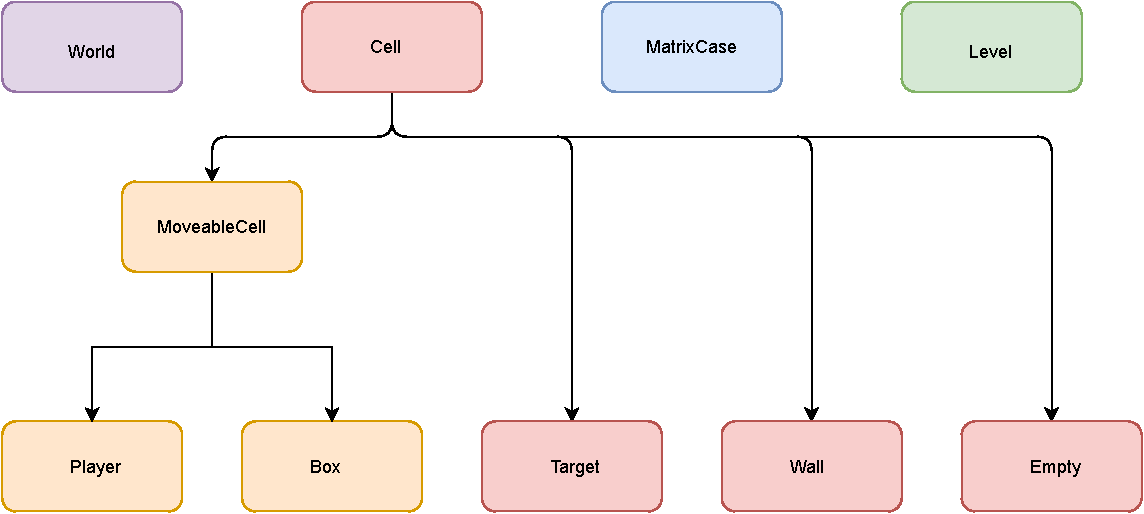
\includegraphics[width=1\textwidth,clip]{images/objects.pdf}

\subsection{Representation d'une map}
Le jeu sokoban nécessite l'implémentation de différentes cellules comme le sol, les murs, les boites, etc.. \\
Une map doit donc pouvoir contenir toutes ces cellules et permettre de les déplacer. Dans ce but, nous avons choisi de représenter une map
par une matrice. Chaque ``case'' de cette matrice est un objet instancié à partir de la classe MatrixCase. Une map est donc une matrice d'objets MatrixCase.\\
Qu'est-ce qu'une MatrixCase ? C'est un objet qui contient deux cellules. En effet une map de sokoban doit permettre la superposition de deux cellules car le joueur ou une boite peuvent se positionner au dessus du sol ou d'une cellule cible.
Schéma d'une MatrixCase :\\

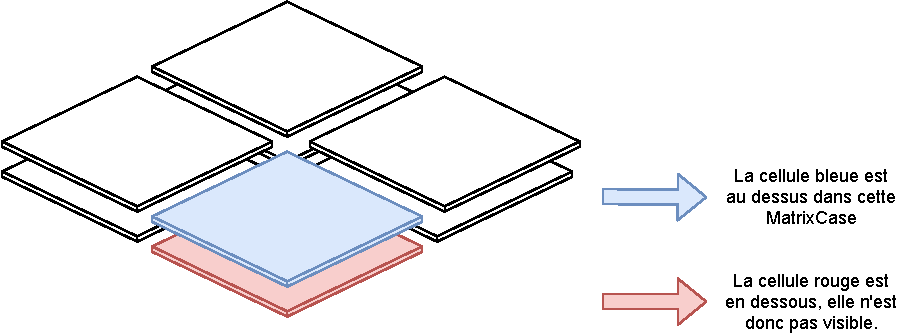
\includegraphics[width=1\textwidth,clip]{images/matrixCase.pdf}

Grâce à cette représentation d'une map, on peut accéder à n'importe quelle cellule de la matrice grâce à ses coordonnées.

\subsection{Chargement d'un niveau}
Un objet instancié à partir de la classe Level du package sokoban.Engine.Objects.Level peut contenir toutes les informations d'un niveau de sokoban,
comme le joueur, le monde dans lequel il évolue, le nom du niveau et sa taille.
La classe Level permet de passer rapidement d'un niveau à l'autre grâce à la méthode setLevel().
Celle-ci prend un nom de map en paramètre et va chercher le fichier xsb correspondant.
Nos fichiers xsb respectent les conventions du sokoban i.e. chaque case du jeu est représenté en texte par un charactère spécifique.
Ce fichier est ensuite tranformé en String par la méthode load de la classe MapLoader.
Ce String est finalement donné en paramètre à la méthode init de la classe Builder qui va pour chaque charactère de ce String créer la case adéquate dans la matrice représentant la map.
Ainsi, toutes les informations nécessaires afin d'afficher un niveau sont disponibles via un objet Level.

\subsection{Déplacements}
Seules les cellules héritant de la classe MoveableCell peuvent être déplacées (voir la hiérarchie des objets).
Le joueur est entièrement controllé par les inputs de l'utilisateur.
Cependant, il ne pourra se déplacer uniquement sous certaines conditions.
En effet le joueur ne doit pas pouvoir traverser ou pousser n'importe quelle cellule.
Voici donc la procédure que nous suivons pour déterminer si oui ou non le joueur peut se déplacer dans la direction donnée par l'utilisateur:\\
Tout d'abord, il faut analyser la case voisine au joueur dans la direction donnée.
\begin{itemize}
	\item Si celle-ci n'est ni traversable ni poussable, alors le joueur ne peut pas se déplacer.
	\item Si elle est traversable et non-poussable, le joueur peut se déplcer.
	\item Si elle est poussable, il faut alors analyser la cellule suivante (toujours dans la même direction).
		\begin{enumerate}
			\item Si la cellule suivante est traversable et non-poussable alors, le joueur peut se déplacer et pousser la cellule devant lui.
			\item Sinon, le joueur ne peut pas se déplacer.
		\end{enumerate}
	\item Dans tous les autres cas, le joueur ne pourra pas se déplacer. 
\end{itemize}
Maintenant que nous avons determiné si le joueur peut se déplacer, on peut déplacer celui-ci dans la matrice représentant la map du niveau et actualiser l'affichage.\\

Cette procédure de déplacement a été implémentée de la façon suivante: \\
Chaque objet représentant une cellule possède les attributs booléens softCollision et hardCollision.
softCollision indique si une cellule est poussable ou non et hardCollision si elle est traversable.\\
Ainsi, en ayant les coordonnées des cellules intervenants dans le déplacement du joueur dans une direction donnée, nous pouvons effectuer les différents tests cités ci-dessus en vérifiant les collisions d'une cellule d'une case précise de la matrice.

\subsection{Génération aléatoire de niveau}

\subsubsection{Backward induction}
Afin d'implémenter la génération aléatoire de niveaux, nous avons commencé par nous renseigner sur les différentes techniques extistantes, notre première idée fut de nous diriger vers une génération procédurale.
Avant de valider ce choix, nous avons questionné notre professeur de mathématique Mr. Brihaye qui nous a conseillé de nous renseigner sur le principe de backward induction.
Après quelques recherches, nous avons décidé d'utiliser cette technique qui semblait plus simple à mettre en place.
La backward induction consiste à partir d'un problème résolu et faire les étapes en marche arrière jusqu'à retrouver un problème initial.
Pour notre sokoban, cela signifie partir d'un niveau résolu et tirer les caisses une à une.
Ainsi, on assure que le niveau sera réalisable puisqu'il suffira de faire les mêmes déplacements dans l'autre sens.\\
Nous avons alors imaginé les étapes nécessaires à la création d'un niveau jouable de sokoban.
\begin{enumerate}
	\item Créer la map vide initiale 
	\item Générer les murs aléatoirement
	\item Placer le joueur sur une case libre aléatoire
	\item Placer aléatoirement et tirer les boites
\end{enumerate}
\begin{itemize}
	\item Etape 1\\
		  La map initiale consiste en une map vide d'une certaine largeur et longueur fermée par des murs.
	\item Etape 2\\
		  Ensuite, les murs sont générés aléatoirements. Pour chaque case de la map on détermine un pourcentage de chance qu'un mur apparaisse.
	\item Etape 3 et 4\\
		  Après avoir placé aléatoirement le joueur, pour chaque boite à placer on va suivre la procédure décrite sur ce schéma :\\
\end{itemize}

\begin{tikzpicture}[font=\small,thick]
 
\node[draw,
    rounded rectangle,
    minimum width=2.5cm,
    minimum height=1cm] (block1) {Faire apparaitre le joueur sur une case aléatoire};
 
\node[draw,
    rounded rectangle, 
    below=of block1,
    minimum width=3.5cm,
    minimum height=1cm] (block2) { Faire apparaitre une caisse sur une case aléatoire };
 
\node[draw,
    rounded rectangle,
    below=of block2,
    minimum width=3.5cm,
    minimum height=1cm] (block3) { Vérifier si un chemin existe du joueur a la caisse };
 
\node[draw,
    rounded rectangle,
    right=of block3,
    minimum width=2.5cm,
    minimum height=1cm] (block4) { Supprimer la caisse };

\node[draw,
    rounded rectangle,
    below=of block3,
    minimum width=2.5cm,
    minimum height=1cm] (block5) { Déplacer le joueur a côté la caisse };
 
\node[draw,
    rounded rectangle,
    below=of block5,
    minimum width=2.5cm,
    minimum height=1cm] (block6) { Tirer la caisse dans des directions aléatoires };
 
% Arrows
    \draw[-latex] (block1) edge (block2);
    \draw[-latex] (block2) edge (block3);
    \draw[-latex, green] (block3) edge (block4);
    \draw[-latex] (block4) |- (block2);
    \draw[-latex, red] (block3) edge (block5);
    \draw[-latex] (block5) edge (block6);
    \draw[-latex] (block6.west) -- ++(-10mm,0) |- (block2.west);

\end{tikzpicture}

\subsubsection{A* path finding}
L'étape 4 de la génération nécessite l'implementation d'un algorithme de pathfinding.\\
Nous avons choisi le très connu A* algorithm pour son adaptabilité et le très grand nombre de ressources disponibles pour son implémentation.\\
cet algorithme consiste à se déplacer d'un point A vers un point B de case en case, en choisissant comme prochaine case celle qui a la plus courte distance vers le point B 
et le point A.

\newpage

\end{document}
